% !TEX program = xelatex
% Options for packages loaded elsewhere
\PassOptionsToPackage{unicode}{hyperref}
\PassOptionsToPackage{hyphens}{url}
%
\documentclass[
  12pt
]{article}
\usepackage[margin=1in]{geometry}
\usepackage{amsmath,amssymb}
\usepackage{graphicx}
\usepackage{tikz}
\usetikzlibrary{arrows.meta,shapes.geometric}
\usepackage{lmodern}
\usepackage{iftex}
\ifPDFTeX
  \usepackage[T1]{fontenc}
  \usepackage[utf8]{inputenc}
  \usepackage{textcomp} % provide euro and other symbols
\else % if luatex or xetex
  \usepackage{unicode-math}
  \defaultfontfeatures{Scale=MatchLowercase}
  \defaultfontfeatures[\rmfamily]{Ligatures=TeX,Scale=1}
\fi
% Use upquote if available, for straight quotes in verbatim environments
\IfFileExists{upquote.sty}{\usepackage{upquote}}{}
\IfFileExists{microtype.sty}{% use microtype if available
  \usepackage[]{microtype}
  \UseMicrotypeSet[protrusion]{basicmath} % disable protrusion for tt fonts
}{}
\makeatletter
\@ifundefined{KOMAClassName}{% if non-KOMA class
  \IfFileExists{parskip.sty}{%
    \usepackage{parskip}
  }{% else
    \setlength{\parindent}{0pt}
    \setlength{\parskip}{6pt plus 2pt minus 1pt}}
}{% if KOMA class
  \KOMAoptions{parskip=half}}
\makeatother
\usepackage{xcolor}
\IfFileExists{xurl.sty}{\usepackage{xurl}}{} % add URL line breaks if available
\IfFileExists{bookmark.sty}{\usepackage{bookmark}}{\usepackage{hyperref}}
\hypersetup{
  hidelinks,
  pdfcreator={LaTeX via pandoc}}
\urlstyle{same} % disable monospaced font for URLs
\usepackage{longtable,booktabs,array}
\usepackage{calc}
\usepackage{needspace} % keep table captions with their tables
% Correct order of tables after \paragraph or \subparagraph
\usepackage{etoolbox}
\makeatletter
\patchcmd\longtable{\par}{\if@noskipsec\mbox{}\fi\par}{}{}
\makeatother
% Allow footnotes in longtable head/foot
\IfFileExists{footnotehyper.sty}{\usepackage{footnotehyper}}{\usepackage{footnote}}
\makesavenoteenv{longtable}
\setlength{\emergencystretch}{3em} % prevent overfull lines
\providecommand{\tightlist}{%
  \setlength{\itemsep}{0pt}\setlength{\parskip}{0pt}}
\setcounter{secnumdepth}{-\maxdimen} % remove section numbering
\ifLuaTeX
  \usepackage{selnolig}  % disable illegal ligatures
\fi

\author{}
\date{}

\begin{document}

\hypertarget{factor-validation-of-activities}{%
\subsection{Factor Validation of Activities}\label{factor-validation-of-activities}}

We examine the empirical correlates of everyday cultural practice by analyzing past-year participation frequencies across 20 distinct activities spanning institutional highbrow arts, commercial entertainment, domestic tasks, and solitary leisure routines. Because these responses are recorded on an ordinal seven-point frequency scale, we estimate principal components on the polychoric correlation matrix using varimax rotation to establish a preliminary exploratory assingment of items to factors. The three-component solution accounts for 63.2 percent of total variance, supported by a Kaiser-Meyer-Olkin sampling adequacy metric of .955 (Table 1).\footnote{Complete responses on all 20 items are available for 1,243 respondents, who form the analytic sample for all measurement models.} 

Substantively, the orthogonal solution uncovers a structural division between public, institutionalized cultural practices and private, domestic routines. Fourteen items coalesce into an expansive public arts factor, uniting traditional fine arts (symphonies, art galleries, theatrical performances) with broadly attended public events (festivals, movies, sporting events). Three items---taking walks, regular exercise or yoga, and literary reading---cluster into an independent solitary leisure dimension. Three remaining practices (gardening, home or automobile repair, and dining at fast-food restaurants) define a residual practical-domestic dimension.\footnote{We also estimated an exploratory factor analysis with direct oblimin rotation on the same polychoric matrix (Table 2). The oblique model fits the 20 items adequately ($\chi^2(133) = 290.8$, $p < .001$, $\text{TLI} = .911$, $\text{RMSEA} = .080$ $[.076, .084]$). Under direct oblimin, the public arts factor remains intact, but the secondary dimensions lose coherence. Assigning items based on highest loadings shifts literary reading, gardening, and home repair onto the arts factor, isolating fast food as a single-item residual. Forcing that assignment into confirmatory models yields inadmissible solutions characterized by negative residual variances and latent correlations exceeding unity. Because the oblique factor correlations in the exploratory solution are small (.19 between arts and leisure, .15 between arts and residual, and .01 between leisure and residual), the orthogonal and oblique orientations differ minimally in practice, and nothing in the data privileges one rotation over the other.}

We evaluate the target structure against more parsimonious alternatives using confirmatory factor analysis with diagonally weighted least squares (WLSMV estimation, N = 1,243; Table 3), which relax the varimax orthogonality assumption by allowing the factors to be correlated. The three-factor model outperforms more parsimonious alternatives. Forcing residual practical items onto the arts factor produces a significant decrement in fit (scaled $\Delta\chi^2(2) = 121.6$, $p < .001$), as does forcing them onto solitary leisure ($\Delta\chi^2(2) = 51.0$, $p < .001$). A single-factor model specifying a generalized omnivorousness dimension performs worst of all ($\Delta\chi^2(3) = 146.4$, $p < .001$). Although the three-factor confirmatory model fits better than any rival ($\text{CFI} = .956$, $\text{RMSEA} = .095$, $\text{SRMR} = .061$), the elevated RMSEA reflects the stringent requirements of independent-clusters simple structure. Cultural practices naturally exhibit secondary cross-loadings across factors that strict zero-loading constraints penalize.

Recognizing that strict zero-loading restrictions can obscure the relational reality of lifestyle practices, we estimate an exploratory structural equation model (ESEM) using target rotation. By anchoring primary loadings to the varimax configuration while permitting items to exhibit small, substantively plausible cross-loadings, the ESEM achieves an good fit to the observed polychoric covariances ($\text{CFI} = .979$, $\text{RMSEA} = .074$ $[.070, .079]$, $\text{SRMR} = .035$), improving over the confirmatory baseline (scaled $\Delta\chi^2(34) = 746.7$, $p < .001$; Table 3).\footnote{Geomin rotation yields identical omnibus fit because rotation does not alter the implied covariance matrix, but it redistributes factor content in an uninterpretable fashion. Under geomin, commercial entertainment (movie theaters, sporting events, dining out) combines with fast food to form the second factor, displacing walking to the third dimension. We retain the varimax targets because they align with the theoretical design of the battery and preserve substantive interpretability.} Latent factor correlations confirm that while these three domains are distinct, they are modestly interrelated; public arts correlates positively with solitary leisure ($r = .36$) and residual domestic practices ($r = .21$), while leisure and residual practices correlate only weakly ($r = .11$; Table 4). As Table 4 shows, all fourteen public arts items maintain primary loadings between .47 and .97. Solitary leisure is anchored firmly by walking (.78) and physical exercise (.42), though exercise also displays a secondary affinity with public cultural engagement (.32). Literary reading functions as the peripheral anchor of this leisure factor across all specifications (.44 in Table 1, .21 in Table 2, and .19 in Table 4), a structural attenuation that proves central to how solitary leisure behaves across alternative operationalizations. Domestic tasks (gardening at .45, home or auto repair at .32) and fast food avoidance ($-.38$) define the residual factor, which also absorbs modest secondary loadings from institutional excursions (museums at .24, historic sites at .23) and outdoor recreation (hiking at .21).\footnote{Several measurement boundaries clarify the scope and reliability of this three-factor solution. First, the residual practical-domestic factor displays modest internal cohesion, registering a McDonald's $\omega$ of .55 and an ordinal $\alpha$ of .31, contrasting with the high internal consistency of public arts ($\alpha = .96$) and the acceptable coherence of solitary leisure ($\alpha = .49$). The disparity between $\omega$ and $\alpha$ for the residual dimension reflects model specification; McDonald's $\omega$ draws upon shared variance within the correlated confirmatory system, whereas Cronbach's $\alpha$ assesses the three items as an isolated scale. Second, low response frequencies in the highest frequency tier across eight items (ranging from two to nine respondents for symphonies, dance performances, and carnivals) introduce potential threshold sparsity into polychoric estimation. Sensitivity analyses collapsing the top two categories across these eight items confirm that the varimax structure remains invariant and yields virtually identical confirmatory fit ($\chi^2(167) = 2049.8$, $\text{CFI} = .955$, $\text{RMSEA} = .095$ $[.092, .099]$), showing that category sparseness does not distort the underlying topology. Third, because direct oblimin rotation merges domestic maintenance with public culture, the empirical standing of the three-factor architecture rests on the mutual reinforcement of varimax target clarity, formal confirmatory testing, and ESEM fit.}


\Needspace{38\baselineskip}
Table 1. Varimax Loadings for the Activity Battery

\begin{longtable}[]{@{}
  >{\raggedright\arraybackslash}p{(\columnwidth - 8\tabcolsep) * \real{0.4200}}
  >{\raggedright\arraybackslash}p{(\columnwidth - 8\tabcolsep) * \real{0.1600}}
  >{\raggedright\arraybackslash}p{(\columnwidth - 8\tabcolsep) * \real{0.1400}}
  >{\raggedright\arraybackslash}p{(\columnwidth - 8\tabcolsep) * \real{0.1400}}
  >{\raggedright\arraybackslash}p{(\columnwidth - 8\tabcolsep) * \real{0.1400}}@{}}
\toprule
Item & Assigned target & Arts & Leisure & Residual \\
Museum & Arts & 0.80 & 0.21 & 0.21 \\
Art gallery & Arts & 0.83 & 0.19 & 0.20 \\
Symphony, orchestra, or opera & Arts & 0.89 & 0.06 & 0.23 \\
Carnival, fair, or amusement park & Arts & 0.83 & 0.13 & 0.01 \\
Music concert or festival & Arts & 0.84 & 0.17 & 0.02 \\
Play or musical & Arts & 0.84 & 0.09 & 0.13 \\
Library & Arts & 0.49 & 0.39 & 0.15 \\
Fancy restaurant & Arts & 0.72 & 0.26 & −0.15 \\
Dance performance & Arts & 0.89 & 0.00 & 0.15 \\
Movie theater & Arts & 0.74 & 0.23 & −0.24 \\
Attend sports & Arts & 0.79 & 0.21 & −0.07 \\
Hiking, camping, or boating & Arts & 0.52 & 0.37 & 0.32 \\
Historic site & Arts & 0.70 & 0.23 & 0.26 \\
Go to festival & Arts & 0.78 & 0.27 & 0.15 \\
Go for a walk & Leisure & −0.14 & 0.87 & 0.07 \\
Exercise or yoga & Leisure & 0.35 & 0.60 & −0.19 \\
Read a novel, poem, or play & Leisure & 0.27 & 0.44 & 0.18 \\
Gardening & Residual & 0.27 & 0.31 & 0.62 \\
Fast food & Residual & 0.21 & 0.22 & −0.66 \\
Home auto repair & Residual & 0.38 & 0.24 & 0.49 \\
\midrule
\endhead
\bottomrule
\end{longtable}

Note. Varimax-rotated component loadings from a principal components analysis (N = 1,243). The assigned target column reports the factor on which each item is assigned in the ESEM targets. The three components together explain 63.2 percent of the variance.

\Needspace{38\baselineskip}
Table 2. Oblimin-Rotated Exploratory Factor Loadings for the Activity Battery

\begin{longtable}[]{@{}
  >{\raggedright\arraybackslash}p{(\columnwidth - 8\tabcolsep) * \real{0.4200}}
  >{\raggedright\arraybackslash}p{(\columnwidth - 8\tabcolsep) * \real{0.1600}}
  >{\raggedright\arraybackslash}p{(\columnwidth - 8\tabcolsep) * \real{0.1400}}
  >{\raggedright\arraybackslash}p{(\columnwidth - 8\tabcolsep) * \real{0.1400}}
  >{\raggedright\arraybackslash}p{(\columnwidth - 8\tabcolsep) * \real{0.1400}}@{}}
\toprule
Item & Assigned target & Arts & Leisure & Residual \\
Museum & Arts & 0.84 & 0.08 & −0.10 \\
Art gallery & Arts & 0.88 & 0.03 & −0.09 \\
Symphony, orchestra, or opera & Arts & 0.95 & −0.14 & −0.11 \\
Carnival, fair, or amusement park & Arts & 0.78 & −0.02 & 0.16 \\
Music concert or festival & Arts & 0.81 & 0.01 & 0.15 \\
Play or musical & Arts & 0.86 & −0.08 & 0.00 \\
Library & Arts & 0.53 & 0.19 & −0.07 \\
Fancy restaurant & Arts & 0.64 & 0.11 & 0.29 \\
Dance performance & Arts & 0.93 & −0.20 & −0.02 \\
Movie theater & Arts & 0.64 & 0.05 & 0.37 \\
Attend sports & Arts & 0.73 & 0.05 & 0.26 \\
Hiking, camping, or boating & Arts & 0.58 & 0.26 & −0.14 \\
Historic site & Arts & 0.74 & 0.12 & −0.12 \\
Go to festival & Arts & 0.80 & 0.12 & 0.01 \\
Go for a walk & Leisure & −0.08 & 0.79 & 0.00 \\
Exercise or yoga & Leisure & 0.31 & 0.37 & 0.25 \\
Read a novel, poem, or play & Leisure & 0.35 & 0.21 & −0.11 \\
Gardening & Residual & 0.42 & 0.22 & −0.34 \\
Fast food & Residual & 0.06 & 0.06 & 0.43 \\
Home auto repair & Residual & 0.48 & 0.16 & −0.23 \\
\midrule
\endhead
\bottomrule
\end{longtable}

Note. Oblimin-rotated pattern loadings from an exploratory factor analysis (WLS estimation, N = 1,243). The EFA fits the 20 items adequately ($\chi^2(133) = 290.8$, $p < .001$, $\text{TLI} = .911$, $\text{RMSEA} = .080$ $[.076, .084]$). The assigned target column reports the varimax assignment used as the ESEM targets. Factor correlations from the oblique solution are .19 (arts and leisure), .15 (arts and residual), and .01 (leisure and residual).

\Needspace{26\baselineskip}
Table 3. Confirmatory and Exploratory Structural Models of the Activity Battery

\begin{longtable}[]{@{}
  >{\raggedright\arraybackslash}p{(\columnwidth - 12\tabcolsep) * \real{0.3000}}
  >{\raggedright\arraybackslash}p{(\columnwidth - 12\tabcolsep) * \real{0.0600}}
  >{\raggedright\arraybackslash}p{(\columnwidth - 12\tabcolsep) * \real{0.1200}}
  >{\raggedright\arraybackslash}p{(\columnwidth - 12\tabcolsep) * \real{0.0800}}
  >{\raggedright\arraybackslash}p{(\columnwidth - 12\tabcolsep) * \real{0.1000}}
  >{\raggedright\arraybackslash}p{(\columnwidth - 12\tabcolsep) * \real{0.1000}}
  >{\raggedright\arraybackslash}p{(\columnwidth - 12\tabcolsep) * \real{0.2400}}@{}}
\toprule
Model & df & Scaled $\chi^2$ & CFI & RMSEA & SRMR & Scaled $\Delta\chi^2$ (df) vs.~three-factor CFA \\
One-factor CFA & 170 & 2225.6 & .952 & .099 & .064 & 146.4 (3), p \textless{} .001 \\
Two-factor CFA, residual merged into arts & 169 & 2199.3 & .952 & .098 & .063 & 121.6 (2), p \textless{} .001 \\
Two-factor CFA, residual merged into leisure & 169 & 2120.8 & .954 & .096 & .062 & 51.0 (2), p \textless{} .001 \\
Three-factor CFA & 167 & 2051.2 & .956 & .095 & .061 & --- \\
ESEM, target rotation & 133 & 1045.1 & .979 & .074 & .035 & 746.7 (34), p \textless{} .001 \\
\midrule
\endhead
\bottomrule
\end{longtable}

Note. N = 1,243. WLSMV estimation. The three-factor CFA is nested within the ESEM's implied covariance class as the case with zero cross-loadings, so the ESEM row reports a scaled difference test against it. The ESEM degrees of freedom reflect its rotation constraints. Latent factor correlations in the three-factor CFA are .76 (arts and leisure), .68 (arts and residual), and .59 (leisure and residual). RMSEA 90\% confidence intervals are {[}.095, .102{]} (one-factor), {[}.095, .102{]} (residual into arts), {[}.093, .100{]} (residual into leisure), {[}.092, .099{]} (three-factor), and {[}.070, .079{]} (ESEM). Scaled difference tests use the Satorra-Bentler scaled statistic with per-model scaling factors.

\Needspace{38\baselineskip}
Table 4. ESEM Loadings with Target Rotation

\begin{longtable}[]{@{}
  >{\raggedright\arraybackslash}p{(\columnwidth - 8\tabcolsep) * \real{0.4200}}
  >{\raggedright\arraybackslash}p{(\columnwidth - 8\tabcolsep) * \real{0.1600}}
  >{\raggedright\arraybackslash}p{(\columnwidth - 8\tabcolsep) * \real{0.1400}}
  >{\raggedright\arraybackslash}p{(\columnwidth - 8\tabcolsep) * \real{0.1400}}
  >{\raggedright\arraybackslash}p{(\columnwidth - 8\tabcolsep) * \real{0.1400}}@{}}
\toprule
Item & Target factor & Arts & Leisure & Residual \\
Museum & Arts & 0.78 & 0.03 & 0.24 \\
Art gallery & Arts & 0.83 & −0.02 & 0.20 \\
Symphony, orchestra, or opera & Arts & 0.95 & −0.22 & 0.11 \\
Carnival, fair, or amusement park & Arts & 0.82 & 0.04 & −0.11 \\
Music concert or festival & Arts & 0.86 & 0.02 & −0.11 \\
Play or musical & Arts & 0.90 & −0.16 & 0.02 \\
Library & Arts & 0.47 & 0.16 & 0.14 \\
Fancy restaurant & Arts & 0.71 & 0.15 & −0.20 \\
Dance performance & Arts & 0.97 & −0.25 & 0.01 \\
Movie theater & Arts & 0.75 & 0.11 & −0.30 \\
Attend sports & Arts & 0.80 & 0.08 & −0.21 \\
Hiking, camping, or boating & Arts & 0.48 & 0.23 & 0.21 \\
Historic site & Arts & 0.65 & 0.11 & 0.23 \\
Go to festival & Arts & 0.78 & 0.10 & 0.04 \\
Go for a walk & Leisure & −0.22 & 0.78 & 0.12 \\
Exercise or yoga & Leisure & 0.32 & 0.42 & −0.17 \\
Read a novel, poem, or play & Leisure & 0.27 & 0.19 & 0.16 \\
Gardening & Residual & 0.23 & 0.17 & 0.45 \\
Fast food & Residual & 0.20 & 0.14 & −0.38 \\
Home auto repair & Residual & 0.34 & 0.14 & 0.32 \\
\midrule
\endhead
\bottomrule
\end{longtable}

Note. Standardized loadings from an ESEM with target rotation (WLSMV, N = 1,243). Factor correlations: arts and leisure .36, arts and residual .21, leisure and residual .11.


\subsection{Factor Validation of Network Composition}\label{factor-validation-of-network-composition}

The tie batteries ask each respondent about the same sixteen kinds of people, once for weak ties and once for strong ties. We expect two dimensions of those networks to carry distinct information. Variety captures how far a respondent's ties extend across ethnic, religious, sexual, and urban-rural positions, and ideological composition captures how those ties sort along liberal and conservative lines. Varimax principal components on each battery's polychoric matrix produce the three-factor sorting used throughout, and we then estimate exploratory structural equation models with target rotation to test that sorting without forcing every cross-loading to zero. Each item loads on its assigned factor and is free to load on the other two. The sorting holds across tie types with two exceptions that matter. Hispanic or Latine people sort to liberal composition in weak networks, where the loading is .54 on liberal and .32 on variety, but to variety in strong networks, where it is .59 on variety and .27 on liberal. Black people split evenly between variety and liberal composition in weak networks (.36 on each) and sort to variety in strong networks (.55 on variety and .18 on liberal). City people sort to liberal composition in both batteries, although the strong-tie loading is nearly tied with variety (.36 and .35).

The target-rotated models fit well on conventional criteria. For weak ties, the ESEM yields CFI = .979, RMSEA = .061 [.056, .067], and SRMR = .029. For strong ties, it yields CFI = .975, RMSEA = .069 [.063, .074], and SRMR = .033. Both improve on the simple-structure confirmatory models, which assign each item to a single factor and fit at CFI = .909 and RMSEA = .111 for weak ties and at CFI = .919 and RMSEA = .106 for strong ties (Table A1). The Satorra-Bentler scaled difference tests are 857.9 on 26 degrees of freedom for weak ties and 693.1 on 26 for strong ties, both p < .001. The gap indicates that zero cross-loadings misdescribe these batteries, and the cross-loadings the ESEM estimates are where much of the substantive content lies.

The largest off-target loadings, up to .41 for weak ties and .36 for strong ties, cluster on the race, place, and religion items. Asian, born-elsewhere, and second-home items carry off-target loadings of .33, .38, and .34 on liberal or conservative composition in weak networks. The Black, Hispanic or Latine, and city items straddle variety and liberal composition in both batteries. White people load .41 on liberal composition in weak ties and .36 in strong ties, alongside primary conservative loadings of .68 and .72. We read these patterns as places where ethnic and urban diversity coincide with political sorting in everyday networks, rather than as sorting errors. The target specification is also partial. In lavaan's partially specified target rotation, zero targets are pulled toward zero rather than pinned, so the surviving off-target loadings are estimates and not constraints, and they should be read as such.

The ESEM factor correlations sit well below the confirmatory ones. For weak ties, variety correlates .52 with liberal composition, .46 with conservative composition, and liberal and conservative composition correlate .47. For strong ties the corresponding values are .48, .54, and .34. The confirmatory models place the same pairs at .81, .62, and .69 for weak ties and .76, .68, and .64 for strong ties. Much of the variety-liberal overlap that drove collinearity in the confirmatory structural models therefore follows from forcing cross-loadings to zero, although the three dimensions remain distinct and positively related.

Reliability is high under the ESEM. Model-implied omega, computed with the cross-loadings included, is .93, .91, and .90 for weak-tie variety, liberal, and conservative composition, and .94, .88, and .88 for strong ties. Restricting the calculation to primary loadings lowers these values to between .84 and .94. The strong-tie liberal factor rests on four items and has an omega of .88 under the ESEM, compared with .79 under the confirmatory model, so it supports more confidence than the earlier measurement models allowed.

We also considered the antonym residuals that improved the confirmatory fit, which pair very liberal with very conservative people, little church with lots of church, and city with rural people. Under the ESEM, the cross-loadings absorb most of that bipolarity. The very liberal and very conservative residual changes sign in weak networks, moving from $-.32$ under the confirmatory model to $+.13$, while the city and rural residual remains negative in both batteries ($-.25$ for weak ties and $-.27$ for strong ties, p = .07). Freeing the antonym residuals alongside the ESEM blocks also makes the strong-tie model numerically unstable, with several path standard errors above 5. We therefore keep the ESEM as specified and report the antonym analysis for the confirmatory models in Table A1. The gender items remain excluded from the network factors, as described in the footnote below.\footnote{Gender items display marked structural ambiguity across both relational domains. In exploratory analyses, knowing women splits nearly equally between the liberal and conservative factors in weak networks (.59 and .60), while knowing men loads heavily on both factors in weak ties (.68 and .57) and on conservative composition in strong ties (.62, alongside a .58 loading on liberal composition). The gender items also generate substantial residual misfit in the confirmatory models. Retaining them lowers confirmatory fit to CFI = .896 and RMSEA = .116 for weak ties and CFI = .918 and RMSEA = .105 for strong ties. Re-estimating our regression models without the four gender items in each battery leaves every substantive finding and significance verdict intact, and no network coefficient shifts by more than .049.}

The structural models in the next subsection use the simple-structure confirmatory factors, which define each network composite by items with zero cross-loadings. The ESEM blocks provide the measurement check, and their structural estimates appear as a robustness analysis in that subsection.\footnote{We do not estimate a joint model that links the weak and strong factors. Such a model requires cross-tie factor correlations near one for the variety factors, and it was not positive definite under either the confirmatory or the target-rotated specification. The separate models are therefore the measurement models for both tie types.}

\Needspace{30\baselineskip}
Table 5. Standardized Loadings from the Target-Rotated ESEM of the Weak-Tie and Strong-Tie Batteries

\begin{tabular*}{\textwidth}{@{\extracolsep{\fill}}>{\raggedright\arraybackslash}p{0.34\textwidth} >{\raggedleft\arraybackslash}p{0.09\textwidth} >{\raggedleft\arraybackslash}p{0.09\textwidth} >{\raggedleft\arraybackslash}p{0.09\textwidth} >{\raggedleft\arraybackslash}p{0.09\textwidth} >{\raggedleft\arraybackslash}p{0.09\textwidth} >{\raggedleft\arraybackslash}p{0.09\textwidth}@{}}
\toprule
 & \multicolumn{3}{c}{Weak ties} & \multicolumn{3}{c}{Strong ties} \\
\cmidrule(lr){2-4}\cmidrule(lr){5-7}
Item & Variety & Liberal & Conservative & Variety & Liberal & Conservative \\
\midrule
Asian people & \textbf{0.61} & 0.33 & $-$0.03 & \textbf{0.73} & 0.15 & $-$0.06 \\
Second home & \textbf{0.50} & $-$0.03 & 0.34 & \textbf{0.56} & $-$0.09 & 0.31 \\
Born elsewhere & \textbf{0.48} & 0.38 & 0.02 & \textbf{0.70} & 0.19 & $-$0.04 \\
Middle Eastern or North African people & \textbf{0.77} & 0.15 & 0.00 & \textbf{0.88} & 0.02 & $-$0.02 \\
Native Hawaiian or Pacific Islander people & \textbf{0.93} & $-$0.04 & $-$0.06 & \textbf{0.93} & $-$0.08 & $-$0.05 \\
American Indian people & \textbf{0.84} & $-$0.12 & 0.06 & \textbf{0.85} & $-$0.14 & 0.09 \\
LGBTQ people & 0.03 & \textbf{0.80} & $-$0.07 & 0.24 & \textbf{0.65} & $-$0.10 \\
Little church & $-$0.11 & \textbf{0.58} & 0.32 & $-$0.07 & \textbf{0.54} & 0.36 \\
Very liberal & $-$0.02 & \textbf{0.78} & 0.05 & 0.08 & \textbf{0.81} & $-$0.01 \\
Hispanic or Latine people & 0.32 & \textbf{0.54} & 0.01 & \textbf{0.59} & 0.27 & $-$0.04 \\
Black people & 0.36 & \textbf{0.36} & 0.16 & \textbf{0.55} & 0.18 & 0.15 \\
City people & 0.30 & \textbf{0.44} & 0.07 & 0.35 & \textbf{0.36} & 0.12 \\
Lots of church & 0.22 & $-$0.02 & \textbf{0.67} & 0.29 & $-$0.09 & \textbf{0.63} \\
Very conservative & 0.11 & $-$0.20 & \textbf{0.90} & 0.14 & $-$0.20 & \textbf{0.81} \\
White people & $-$0.19 & 0.41 & \textbf{0.68} & $-$0.15 & 0.36 & \textbf{0.72} \\
Rural people & $-$0.07 & 0.11 & \textbf{0.61} & $-$0.05 & 0.16 & \textbf{0.60} \\
\bottomrule
\end{tabular*}

Note. Standardized loadings from exploratory structural equation models with target rotation (WLSMV, polychoric; N = 1,258 per battery). Bold entries are the primary loadings from the target, and all other loadings are estimated rather than fixed at zero. Gender items are excluded. Factor correlations are .52 (variety and liberal), .46 (variety and conservative), and .47 (liberal and conservative) for weak ties, and .48, .54, and .34 in the same order for strong ties. Item labels are abbreviated from the variable names.


\subsection{Structural Models of Activity Participation}\label{structural-models-of-activity-participation}

To evaluate how network variety and ideological composition relate to cultural participation, we estimate structural equation models separately across weak and strong ties on the confirmatory network and activity factors defined above. Each system incorporates the three validated network dimensions (variety, liberal composition, and conservative composition), the three activity domains (public arts, solitary leisure, and practical-domestic residual), and comprehensive sociodemographic controls. Gender, race and ethnicity, and childhood arts exposure enter as specified in our regression models; age enters linearly in years. Education is specified as a single ordinal scale ranging from high school or less (1) to graduate credentials (4), capturing monotonic human-capital accumulation across adjacent educational tiers. Household income and political conservatism (ranging from 1 for very liberal to 7 for very conservative) enter as linear predictors. Estimated on complete cases (N = 1,227) using weighted least squares with mean and variance adjustment (WLSMV), both models converge cleanly, yield positive definite covariance matrices, and fit the data well ($\text{CFI} = .906$, $\text{RMSEA} = .055$ $[.053, .057]$, $\text{SRMR} = .061$ for weak ties; $\text{CFI} = .903$, $\text{RMSEA} = .056$ $[.054, .058]$, $\text{SRMR} = .059$ for strong ties).

The structural estimates reveal that network variety functions as the central relational channel for public arts attendance across both weak ($\beta = .85$, $p < .001$) and strong ($\beta = .68$, $p < .001$) ties (Table 6). Once network variety is held constant, liberal network composition exhibits a significant negative net association with public arts participation ($-.58$, $p < .001$ for weak ties; $-.27$, $p < .001$ for strong ties). Conservative composition, by contrast, shows no discernible relationship with public arts engagement in either relational sphere. Wald tests of joint significance confirm that network factors exert a collective influence on arts participation ($\chi^2(3) = 137.1$ for weak ties; $\chi^2(3) = 207.3$ for strong ties, both $p < .001$), with a parallel configuration emerging for practical domestic activities.

Solitary leisure follows a different pattern, which marks the limits of network influence. Unlike public arts attendance, which requires social coordination and carries public signaling value, solitary routines such as walking, reading, and personal fitness unfold in private settings. Consequently, network variety plays no role in driving solitary leisure ($\beta = .06$ for weak ties; $\beta = -.01$ for strong ties). Only liberal composition displays a modest positive association with solitary routines ($\beta = .26$, $p = .10$ for weak ties; $\beta = .26$, $p = .02$ for strong ties), and block tests indicate joint network associations despite the weakness of the individual paths.

The substantial overlap between weak-tie variety and liberal composition warrants careful substantive interpretation. After conditioning on covariates, these two dimensions correlate at .83, yielding variance inflation factors of 3.4 for variety and 5.5 for liberal composition. In bivariate specifications that omit variety, the association between liberal composition and arts attendance is positive; it turns negative only when estimated jointly with network breadth. The resulting suppression dynamic clarifies a central theoretical puzzle; in contemporary American society, demographic diversity and progressive political environments frequently intersect. Bivariate models misattribute the cultural benefits of demographic bridging to progressive homophily. When structural variety is held constant, however, an insular concentration of progressive ties does not expand cultural practice---it constrains it. Broad network bridges across diverse social positions, rather than ideological sorting into progressive enclaves, provide the relational capital that sustains public cultural engagement. Conversely, holding liberal composition constant reveals the full power of structural variety, elevating its coefficient from .36 in isolation to 1.08 in joint estimation.

Sociodemographic patterns reinforce these relational dynamics across both models (Tables 7--10). Educational attainment predicts public arts attendance, solitary leisure, and practical domestic tasks, while expanding network variety across weak ($\beta = .29$, $p < .001$) and strong ($\beta = .27$, $p < .001$) ties. Asian American and Pacific Islander respondents report lower public arts participation relative to White respondents in both models ($\beta = -.12$ weak, $-.10$ strong, both $p < .001$). Minoritized racial and ethnic groups (Black, Hispanic or Latine, AAPI, and multiracial respondents) consistently maintain fewer conservative ties than White respondents. Political conservatism predicts conservative network sorting and depresses liberal ties across both relational domains.

Sensitivity checks confirm the stability of these structural estimates. Freeing the three antonym residual covariances in the confirmatory models (Table A1) shifts standardized network paths by at most .03, leaving every substantive pattern and significance threshold unchanged. Similarly, omitting conservative composition from the arts equation alters the remaining coefficients only modestly.

We also re-estimated the network-to-activity paths with the target-rotated ESEM blocks in place of the confirmatory network factors, keeping the activity factors and covariates unchanged.\footnote{We do not report covariate paths onto the ESEM blocks. In lavaan 0.7-3, regressions of covariates onto target-rotated factors produced coefficients whose signs contradicted the item-level associations, and changing the exogeneity specification did not resolve the problem. The network-to-activity estimates reported here come from models that include the same covariates.} The weak-tie variety and liberal paths keep their direction and significance, at .55 and $-.36$ in standardized form, against .85 and $-.58$ under the confirmatory factors, and the weak-tie conservative path stays null. The weak-tie joint test for solitary leisure remains significant ($\chi^2(3) = 15.9$, p = .001). The strong-tie variety path remains significant at .58 (p = .005). The strong-tie liberal path on arts shrinks to $-.24$ and is not significant (p = .65), and the strong-tie joint test for solitary leisure falls to $\chi^2(3) = 6.4$, p = .10. The weak-tie composition effects are therefore more modest than the confirmatory estimates suggest, and the strong-tie liberal coefficient should not be read as a firm finding. The residual factor paths are null under both measurements.

Several methodological boundaries contextualize these structural findings. The practical-domestic residual factor exhibits low internal reliability ($\omega = .55$), indicating that its structural paths should be interpreted with caution. In addition, because these survey data are cross-sectional, the structural models identify patterns of relational association rather than causal trajectories; the network-mediated pathways illuminate the empirical extent to which social ties channel demographic advantages, without assuming that network configurations are exogenous to cultural dispositions. Finally, estimating separate structural systems for weak and strong ties preserves empirical identification at the expense of modeling cross-tie interdependencies simultaneously.

Table 6. Standardized Network-to-Activity Paths from the Separate Weak-Tie and Strong-Tie Structural Models

\begin{tabular*}{\textwidth}{@{\extracolsep{\fill}}>{\raggedright\arraybackslash}p{0.40\textwidth} >{\raggedleft\arraybackslash}p{0.16\textwidth} >{\raggedleft\arraybackslash}p{0.16\textwidth} >{\raggedleft\arraybackslash}p{0.16\textwidth}@{}}
\toprule
Network factor & Arts & Solitary leisure & Residual \\
\midrule
Weak variety & \hphantom{$-$}0.85***\hphantom{} & \hphantom{$-$}0.06\hphantom{***} & \hphantom{$-$}0.86***\hphantom{} \\
Weak liberal & $-$0.58***\hphantom{} & \hphantom{$-$}0.26\hphantom{***} & $-$0.89***\hphantom{} \\
Weak conservative & \hphantom{$-$}0.09\hphantom{***} & $-$0.07\hphantom{***} & \hphantom{$-$}0.47***\hphantom{} \\
Strong variety & \hphantom{$-$}0.68***\hphantom{} & $-$0.01\hphantom{***} & \hphantom{$-$}0.47***\hphantom{} \\
Strong liberal & $-$0.27***\hphantom{} & \hphantom{$-$}0.26*\hphantom{**} & $-$0.33**\hphantom{*} \\
Strong conservative & $-$0.02\hphantom{***} & \hphantom{$-$}0.01\hphantom{***} & \hphantom{$-$}0.23*\hphantom{**} \\
\bottomrule
\end{tabular*}

Note. Standardized coefficients from separate WLSMV structural models for weak ties and strong ties (N = 1,227 each). * p < .05, ** p < .01, *** p < .001. Each model includes gender, education (single ordinal variable), childhood arts, income, age in years, race and ethnicity, and political ideology as predictors of all network and activity factors. The weak-tie liberal and variety coefficients on arts are estimated jointly and should be read as conditional on each other.

Table 7. Sociodemographic Predictors of Weak-Tie Network Composition Factors

\begin{tabular*}{\textwidth}{@{\extracolsep{\fill}}>{\raggedright\arraybackslash}p{0.40\textwidth} >{\raggedleft\arraybackslash}p{0.16\textwidth} >{\raggedleft\arraybackslash}p{0.16\textwidth} >{\raggedleft\arraybackslash}p{0.16\textwidth}@{}}
\toprule
Predictor & Variety & Liberal & Conservative \\
\midrule
Age (years) & $-$0.11***\hphantom{} & $-$0.04\hphantom{***} & \hphantom{$-$}0.00\hphantom{***} \\
Education (ordinal, 1 to 4) & \hphantom{$-$}0.29***\hphantom{} & \hphantom{$-$}0.13***\hphantom{} & \hphantom{$-$}0.14***\hphantom{} \\
Childhood arts exposure & \hphantom{$-$}0.26***\hphantom{} & \hphantom{$-$}0.17***\hphantom{} & \hphantom{$-$}0.10**\hphantom{*} \\
Household income & \hphantom{$-$}0.09**\hphantom{*} & \hphantom{$-$}0.07*\hphantom{**} & \hphantom{$-$}0.10**\hphantom{*} \\
Political ideology (1 to 7) & \hphantom{$-$}0.03\hphantom{***} & $-$0.27***\hphantom{} & \hphantom{$-$}0.26***\hphantom{} \\
Man (ref. woman) & \hphantom{$-$}0.00\hphantom{***} & $-$0.07*\hphantom{**} & $-$0.09**\hphantom{*} \\
Non-binary/trans (ref. woman) & $-$0.04\hphantom{***} & $-$0.05\hphantom{***} & $-$0.08**\hphantom{*} \\
Black (ref. White) & \hphantom{$-$}0.05\hphantom{***} & \hphantom{$-$}0.03\hphantom{***} & $-$0.15***\hphantom{} \\
Hispanic or Latine (ref. White) & \hphantom{$-$}0.05\hphantom{***} & \hphantom{$-$}0.06*\hphantom{**} & $-$0.14***\hphantom{} \\
AAPI (ref. White) & \hphantom{$-$}0.07**\hphantom{*} & $-$0.02\hphantom{***} & $-$0.16***\hphantom{} \\
Mixed/other (ref. White) & \hphantom{$-$}0.06*\hphantom{**} & \hphantom{$-$}0.04\hphantom{***} & $-$0.11***\hphantom{} \\
\bottomrule
\end{tabular*}

Note. Standardized coefficients from the weak-tie structural model (N = 1,227). * p < .05, ** p < .01, *** p < .001. Reference categories are shown in parentheses. Education is a single ordinal variable. Political ideology ranges from 1 (very liberal) to 7 (very conservative).


Table 8. Sociodemographic Predictors of Strong-Tie Network Composition Factors

\begin{tabular*}{\textwidth}{@{\extracolsep{\fill}}>{\raggedright\arraybackslash}p{0.40\textwidth} >{\raggedleft\arraybackslash}p{0.16\textwidth} >{\raggedleft\arraybackslash}p{0.16\textwidth} >{\raggedleft\arraybackslash}p{0.16\textwidth}@{}}
\toprule
Predictor & Variety & Liberal & Conservative \\
\midrule
Age (years) & $-$0.11***\hphantom{} & $-$0.03\hphantom{***} & $-$0.01\hphantom{***} \\
Education (ordinal, 1 to 4) & \hphantom{$-$}0.27***\hphantom{} & \hphantom{$-$}0.18***\hphantom{} & \hphantom{$-$}0.17***\hphantom{} \\
Childhood arts exposure & \hphantom{$-$}0.29***\hphantom{} & \hphantom{$-$}0.22***\hphantom{} & \hphantom{$-$}0.13***\hphantom{} \\
Household income & \hphantom{$-$}0.01\hphantom{***} & \hphantom{$-$}0.09**\hphantom{*} & \hphantom{$-$}0.03\hphantom{***} \\
Political ideology (1 to 7) & \hphantom{$-$}0.07*\hphantom{**} & $-$0.32***\hphantom{} & \hphantom{$-$}0.35***\hphantom{} \\
Man (ref. woman) & $-$0.01\hphantom{***} & $-$0.08**\hphantom{*} & $-$0.09**\hphantom{*} \\
Non-binary/trans (ref. woman) & $-$0.03\hphantom{***} & $-$0.02\hphantom{***} & $-$0.05\hphantom{***} \\
Black (ref. White) & \hphantom{$-$}0.12***\hphantom{} & $-$0.02\hphantom{***} & $-$0.14***\hphantom{} \\
Hispanic or Latine (ref. White) & \hphantom{$-$}0.08**\hphantom{*} & \hphantom{$-$}0.00\hphantom{***} & $-$0.11***\hphantom{} \\
AAPI (ref. White) & \hphantom{$-$}0.02\hphantom{***} & $-$0.08**\hphantom{*} & $-$0.21***\hphantom{} \\
Mixed/other (ref. White) & \hphantom{$-$}0.04\hphantom{***} & $-$0.04\hphantom{***} & $-$0.16***\hphantom{} \\
\bottomrule
\end{tabular*}

Note. Standardized coefficients from the strong-tie structural model (N = 1,227). * p < .05, ** p < .01, *** p < .001. Reference categories are shown in parentheses. Education is a single ordinal variable. Political ideology ranges from 1 (very liberal) to 7 (very conservative).


Table 9. Sociodemographic Predictors of Weak-Tie Activity Factors

\begin{tabular*}{\textwidth}{@{\extracolsep{\fill}}>{\raggedright\arraybackslash}p{0.40\textwidth} >{\raggedleft\arraybackslash}p{0.16\textwidth} >{\raggedleft\arraybackslash}p{0.16\textwidth} >{\raggedleft\arraybackslash}p{0.16\textwidth}@{}}
\toprule
Predictor & Arts & Solitary leisure & Residual \\
\midrule
Age (years) & $-$0.08**\hphantom{*} & $-$0.15***\hphantom{} & \hphantom{$-$}0.14**\hphantom{*} \\
Education (ordinal, 1 to 4) & \hphantom{$-$}0.20***\hphantom{} & \hphantom{$-$}0.32***\hphantom{} & \hphantom{$-$}0.06\hphantom{***} \\
Childhood arts exposure & \hphantom{$-$}0.16***\hphantom{} & \hphantom{$-$}0.16***\hphantom{} & \hphantom{$-$}0.07\hphantom{***} \\
Household income & \hphantom{$-$}0.04\hphantom{***} & \hphantom{$-$}0.11**\hphantom{*} & $-$0.02\hphantom{***} \\
Political ideology (1 to 7) & $-$0.12*\hphantom{**} & $-$0.01\hphantom{***} & $-$0.27**\hphantom{*} \\
Man (ref. woman) & $-$0.04\hphantom{***} & $-$0.10*\hphantom{**} & $-$0.01\hphantom{***} \\
Non-binary/trans (ref. woman) & \hphantom{$-$}0.02\hphantom{***} & $-$0.02\hphantom{***} & \hphantom{$-$}0.03\hphantom{***} \\
Black (ref. White) & \hphantom{$-$}0.04\hphantom{***} & $-$0.03\hphantom{***} & $-$0.01\hphantom{***} \\
Hispanic or Latine (ref. White) & \hphantom{$-$}0.03\hphantom{***} & $-$0.04\hphantom{***} & \hphantom{$-$}0.05\hphantom{***} \\
AAPI (ref. White) & $-$0.12***\hphantom{} & $-$0.07\hphantom{***} & $-$0.02\hphantom{***} \\
Mixed/other (ref. White) & $-$0.05\hphantom{***} & \hphantom{$-$}0.00\hphantom{***} & \hphantom{$-$}0.07\hphantom{***} \\
\bottomrule
\end{tabular*}

Note. Standardized coefficients from the weak-tie structural model in Table 7 (N = 1,227). * p < .05, ** p < .01, *** p < .001. The activity equations also include the three weak-tie network factors, whose coefficients are reported in Table 6.


Table 10. Sociodemographic Predictors of Strong-Tie Activity Factors

\begin{tabular*}{\textwidth}{@{\extracolsep{\fill}}>{\raggedright\arraybackslash}p{0.40\textwidth} >{\raggedleft\arraybackslash}p{0.16\textwidth} >{\raggedleft\arraybackslash}p{0.16\textwidth} >{\raggedleft\arraybackslash}p{0.16\textwidth}@{}}
\toprule
Predictor & Arts & Solitary leisure & Residual \\
\midrule
Age (years) & $-$0.09***\hphantom{} & $-$0.17***\hphantom{} & \hphantom{$-$}0.12**\hphantom{*} \\
Education (ordinal, 1 to 4) & \hphantom{$-$}0.25***\hphantom{} & \hphantom{$-$}0.32***\hphantom{} & \hphantom{$-$}0.16***\hphantom{} \\
Childhood arts exposure & \hphantom{$-$}0.16***\hphantom{} & \hphantom{$-$}0.16***\hphantom{} & \hphantom{$-$}0.10*\hphantom{**} \\
Household income & \hphantom{$-$}0.10***\hphantom{} & \hphantom{$-$}0.11*\hphantom{**} & \hphantom{$-$}0.07\hphantom{***} \\
Political ideology (1 to 7) & $-$0.04\hphantom{***} & $-$0.01\hphantom{***} & $-$0.10\hphantom{***} \\
Man (ref. woman) & $-$0.02\hphantom{***} & $-$0.09*\hphantom{**} & \hphantom{$-$}0.01\hphantom{***} \\
Non-binary/trans (ref. woman) & \hphantom{$-$}0.02\hphantom{***} & $-$0.03\hphantom{***} & \hphantom{$-$}0.02\hphantom{***} \\
Black (ref. White) & $-$0.04\hphantom{***} & \hphantom{$-$}0.00\hphantom{***} & $-$0.09*\hphantom{**} \\
Hispanic or Latine (ref. White) & $-$0.03\hphantom{***} & $-$0.01\hphantom{***} & $-$0.04\hphantom{***} \\
AAPI (ref. White) & $-$0.10***\hphantom{} & $-$0.04\hphantom{***} & \hphantom{$-$}0.00\hphantom{***} \\
Mixed/other (ref. White) & $-$0.07**\hphantom{*} & \hphantom{$-$}0.03\hphantom{***} & \hphantom{$-$}0.04\hphantom{***} \\
\bottomrule
\end{tabular*}

Note. Standardized coefficients from the strong-tie structural model in Table 8 (N = 1,227). * p < .05, ** p < .01, *** p < .001. The activity equations also include the three strong-tie network factors, whose coefficients are reported in Table 6.


Decomposing total associations into direct and network-mediated pathways reveals how stratification advantages and political dispositions are translated into cultural practice (Tables 11 and 12; Figures 5--10). Educational attainment exhibits the strongest total association with public arts participation across both relational models ($\beta = .38$, $p < .001$). In weak networks, nearly half of this educational advantage (network-mediated effect $= .18$, $p < .001$) is channeled through social networks, driven primarily by network variety (.25) and partially counterbalanced by liberal composition ($-.07$). In strong networks, the network-mediated share accounts for roughly one-third of the total association (.13, $p < .001$), operating through network variety (.18) and liberal composition ($-.05$). By contrast, the educational gradient for solitary leisure operates almost entirely as a direct effect ($\beta = .32$, $p < .001$ in weak ties), with network mediation playing virtually no role (.04, not significant). In strong networks, education exerts a modest indirect path on leisure through liberal composition (.05, $p = .04$). For practical domestic activities, education operates predominantly through network pathways (.20 in weak ties; .11 in strong ties), fueled by network variety (.25 and .13) and tempered by liberal composition ($-.11$ and $-.06$), with a modest positive contribution from conservative ties in weak networks (.07).

Childhood arts socialization displays a parallel dual pathway structure. Early exposure to the arts yields a total association of .29 ($p < .001$) with adult arts attendance across both tie types. Approximately 45 percent of this total effect (network-mediated effect $= .13$, $p < .001$) operates indirectly through adult network formation, almost exclusively through the construction of diverse network ties (.22 for weak ties; .19 for strong ties), offset slightly by liberal composition ($-.10$ and $-.06$). The direct socialization effect remains substantial ($\beta = .16$, $p < .001$). Childhood socialization also exerts significant network-mediated effects on solitary leisure (.06 across both tie types) and on practical domestic tasks (.12 in weak ties; .09 in strong ties). In weak networks, the indirect leisure effect reflects the joint precision of negatively covarying path estimates rather than a single dominant channel; in strong networks, it is mediated specifically by liberal composition (.06, $p = .03$).

Political conservatism exhibits a suppression dynamic. The total association between conservatism and public arts attendance is modest and positive (.09, $p < .001$ across both tie types), but this net estimate conceals opposing direct and indirect forces. In weak ties, conservative respondents exhibit a significant negative direct orientation toward public arts participation ($-.12$, $p < .05$). That negative direct inclination is more than offset by a substantial positive network-mediated effect (.20, $p < .001$), flowing primarily through the liberal composition channel (.16), with a small contribution from network variety (.02). Because conservative individuals maintain fewer liberal acquaintances, they bypass the negative net constraint that progressive network insularity imposes on arts participation. In strong ties, the direct association is negligible ($-.04$, not significant), while the network-mediated path remains positive (.13, $p < .001$). A similar dynamic governs practical domestic activities in weak networks, where a negative direct association ($-.27$, $p < .01$) is overridden by positive network mediation (.39, $p < .001$) running through both liberal (.24) and conservative (.12) composition channels. For solitary leisure, political conservatism displays a negative total association ($-.10$ in weak ties; $-.09$ in strong ties), but aggregate network-mediated effects do not reach significance in either domain, despite a modest negative indirect path through strong-tie liberal composition ($-.08$, $p = .03$).

The path decompositions illuminate the relational pathways through which stratification shapes cultural practice, under standard cross-sectional mediation assumptions that condition on our observed demographic covariates. The network-mediated effects quantify the proportion of total demographic associations channeled through social network configurations, clarifying the relational mechanisms that link social origins to everyday cultural lifestyles.

Figure 5. Paths from Education to Arts Participation, Weak Ties

\begin{center}
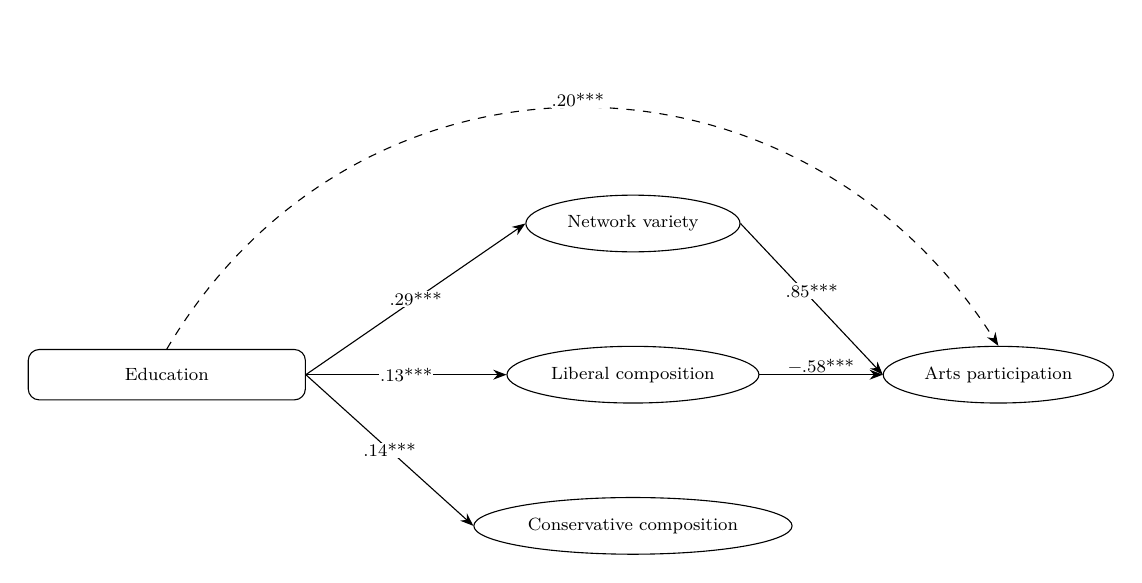
\begin{tikzpicture}[>=Stealth, font=\footnotesize, scale=0.8, transform shape,
  box/.style={draw, rounded corners, align=center, minimum width=4.4cm, minimum height=0.8cm},
  lat/.style={draw, ellipse, align=center, minimum width=3.4cm, minimum height=0.9cm},
  lab/.style={fill=white, inner sep=0.5pt, font=\footnotesize}]
\node[box] (x) at (0,0) {Education};
\node[lat] (wv) at (7.4,2.4) {Network variety};
\node[lat] (wl) at (7.4,0) {Liberal composition};
\node[lat] (wc) at (7.4,-2.4) {Conservative composition};
\node[lat] (act) at (13.2,0) {Arts participation};
\draw[->] (x.east) -- node[lab, pos=0.5] {.29***} (wv.west);
\draw[->] (x.east) -- node[lab, pos=0.5] {.13***} (wl.west);
\draw[->] (x.east) -- node[lab, pos=0.5] {.14***} (wc.west);
\draw[->] (wv.east) -- node[lab, pos=0.5, above] {.85***} (act.west);
\draw[->] (wl.east) -- node[lab, pos=0.5, above] {$-$.58***} (act.west);
\draw[->, dashed] (x.north) .. controls (3,5.5) and (10,5.5) .. node[lab, pos=0.5, above] {.20***} (act.north);
\end{tikzpicture}
\end{center}

Note. Standardized coefficients from the weak-tie structural model (N = 1,227). Solid arrows are paths through the network factors, dashed arrows are direct paths, and only paths significant at p < .05 are drawn. Asterisks follow Table 6.

Figure 6. Paths from Childhood Arts Exposure to Arts Participation, Weak Ties

\begin{center}
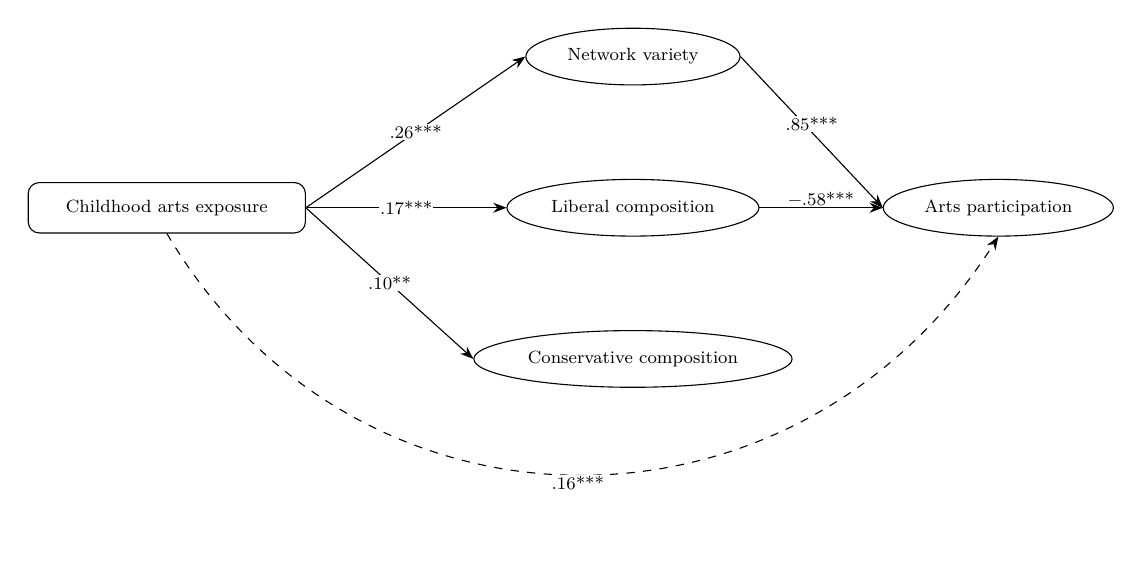
\begin{tikzpicture}[>=Stealth, font=\footnotesize, scale=0.8, transform shape,
  box/.style={draw, rounded corners, align=center, minimum width=4.4cm, minimum height=0.8cm},
  lat/.style={draw, ellipse, align=center, minimum width=3.4cm, minimum height=0.9cm},
  lab/.style={fill=white, inner sep=0.5pt, font=\footnotesize}]
\node[box] (x) at (0,0) {Childhood arts exposure};
\node[lat] (wv) at (7.4,2.4) {Network variety};
\node[lat] (wl) at (7.4,0) {Liberal composition};
\node[lat] (wc) at (7.4,-2.4) {Conservative composition};
\node[lat] (act) at (13.2,0) {Arts participation};
\draw[->] (x.east) -- node[lab, pos=0.5] {.26***} (wv.west);
\draw[->] (x.east) -- node[lab, pos=0.5] {.17***} (wl.west);
\draw[->] (x.east) -- node[lab, pos=0.5] {.10**} (wc.west);
\draw[->] (wv.east) -- node[lab, pos=0.5, above] {.85***} (act.west);
\draw[->] (wl.east) -- node[lab, pos=0.5, above] {$-$.58***} (act.west);
\draw[->, dashed] (x.south) .. controls (3,-5.5) and (10,-5.5) .. node[lab, pos=0.5, below] {.16***} (act.south);
\end{tikzpicture}
\end{center}

Note. Standardized coefficients from the weak-tie structural model (N = 1,227). Solid arrows are paths through the network factors, dashed arrows are direct paths, and only paths significant at p < .05 are drawn. Asterisks follow Table 6.

Figure 7. Paths from Political Conservatism to Arts Participation, Weak Ties

\begin{center}
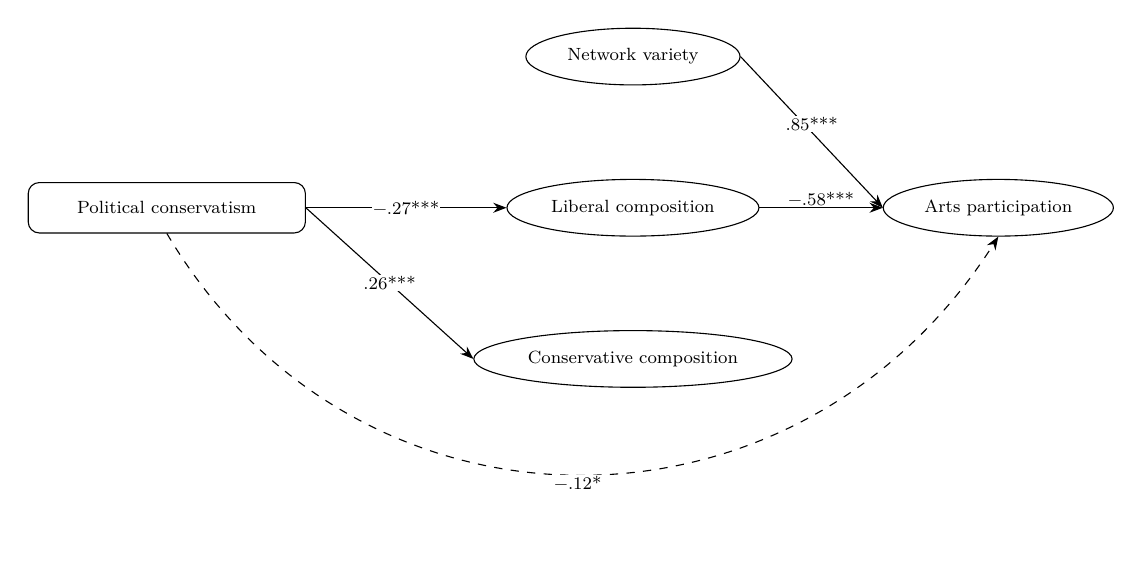
\begin{tikzpicture}[>=Stealth, font=\footnotesize, scale=0.8, transform shape,
  box/.style={draw, rounded corners, align=center, minimum width=4.4cm, minimum height=0.8cm},
  lat/.style={draw, ellipse, align=center, minimum width=3.4cm, minimum height=0.9cm},
  lab/.style={fill=white, inner sep=0.5pt, font=\footnotesize}]
\node[box] (x) at (0,0) {Political conservatism};
\node[lat] (wv) at (7.4,2.4) {Network variety};
\node[lat] (wl) at (7.4,0) {Liberal composition};
\node[lat] (wc) at (7.4,-2.4) {Conservative composition};
\node[lat] (act) at (13.2,0) {Arts participation};
\draw[->] (x.east) -- node[lab, pos=0.5] {$-$.27***} (wl.west);
\draw[->] (x.east) -- node[lab, pos=0.5] {.26***} (wc.west);
\draw[->] (wv.east) -- node[lab, pos=0.5, above] {.85***} (act.west);
\draw[->] (wl.east) -- node[lab, pos=0.5, above] {$-$.58***} (act.west);
\draw[->, dashed] (x.south) .. controls (3,-5.5) and (10,-5.5) .. node[lab, pos=0.5, below] {$-$.12*} (act.south);
\end{tikzpicture}
\end{center}

Note. Standardized coefficients from the weak-tie structural model (N = 1,227). Solid arrows are paths through the network factors, dashed arrows are direct paths, and only paths significant at p < .05 are drawn. Asterisks follow Table 6.

Figure 8. Paths from Education to Arts Participation, Strong Ties

\begin{center}
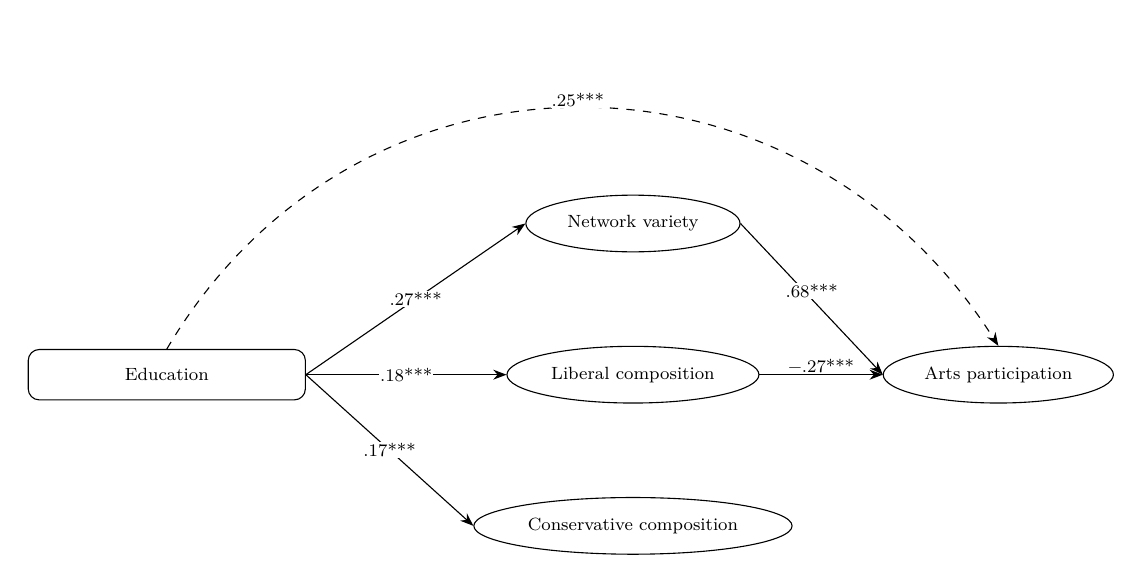
\begin{tikzpicture}[>=Stealth, font=\footnotesize, scale=0.8, transform shape,
  box/.style={draw, rounded corners, align=center, minimum width=4.4cm, minimum height=0.8cm},
  lat/.style={draw, ellipse, align=center, minimum width=3.4cm, minimum height=0.9cm},
  lab/.style={fill=white, inner sep=0.5pt, font=\footnotesize}]
\node[box] (x) at (0,0) {Education};
\node[lat] (wv) at (7.4,2.4) {Network variety};
\node[lat] (wl) at (7.4,0) {Liberal composition};
\node[lat] (wc) at (7.4,-2.4) {Conservative composition};
\node[lat] (act) at (13.2,0) {Arts participation};

\draw[->] (x.east) -- node[lab, pos=0.5] {.27***} (wv.west);
\draw[->] (x.east) -- node[lab, pos=0.5] {.18***} (wl.west);
\draw[->] (x.east) -- node[lab, pos=0.5] {.17***} (wc.west);
\draw[->] (wv.east) -- node[lab, pos=0.5, above] {.68***} (act.west);
\draw[->] (wl.east) -- node[lab, pos=0.5, above] {$-$.27***} (act.west);
\draw[->, dashed] (x.north) .. controls (3,5.5) and (10,5.5) .. node[lab, pos=0.5, above] {.25***} (act.north);
\end{tikzpicture}
\end{center}

Note. Standardized coefficients from the strong-tie structural model (N = 1,227). Solid arrows are paths through the network factors, dashed arrows are direct paths, and only paths significant at p < .05 are drawn. Asterisks follow Table 6.

Figure 9. Paths from Childhood Arts Exposure to Arts Participation, Strong Ties

\begin{center}
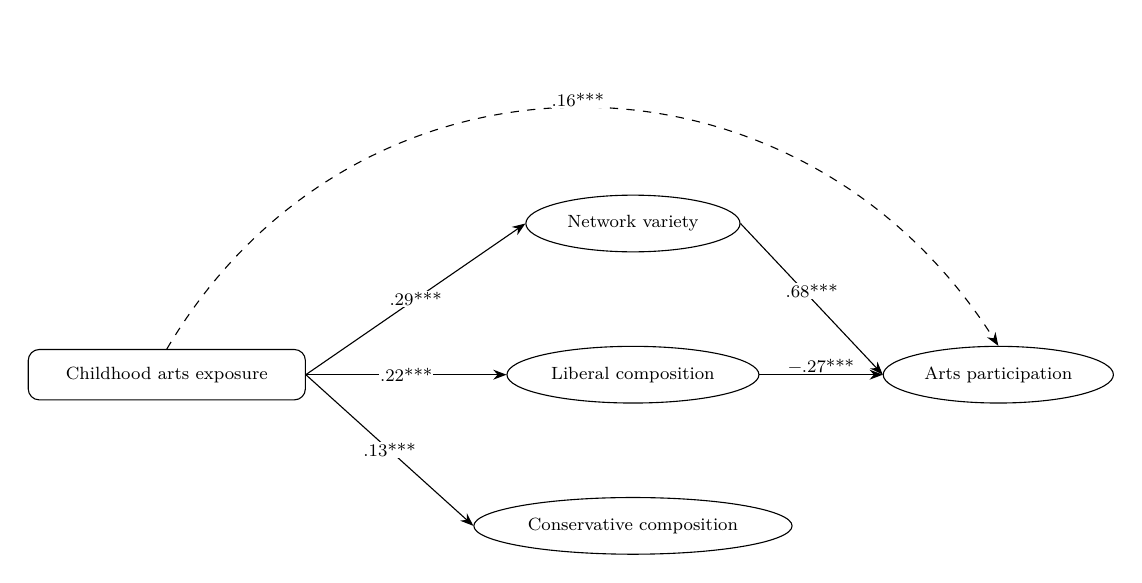
\begin{tikzpicture}[>=Stealth, font=\footnotesize, scale=0.8, transform shape,
  box/.style={draw, rounded corners, align=center, minimum width=4.4cm, minimum height=0.8cm},
  lat/.style={draw, ellipse, align=center, minimum width=3.4cm, minimum height=0.9cm},
  lab/.style={fill=white, inner sep=0.5pt, font=\footnotesize}]
\node[box] (x) at (0,0) {Childhood arts exposure};
\node[lat] (wv) at (7.4,2.4) {Network variety};
\node[lat] (wl) at (7.4,0) {Liberal composition};
\node[lat] (wc) at (7.4,-2.4) {Conservative composition};
\node[lat] (act) at (13.2,0) {Arts participation};

\draw[->] (x.east) -- node[lab, pos=0.5] {.29***} (wv.west);
\draw[->] (x.east) -- node[lab, pos=0.5] {.22***} (wl.west);
\draw[->] (x.east) -- node[lab, pos=0.5] {.13***} (wc.west);
\draw[->] (wv.east) -- node[lab, pos=0.5, above] {.68***} (act.west);
\draw[->] (wl.east) -- node[lab, pos=0.5, above] {$-$.27***} (act.west);
\draw[->, dashed] (x.north) .. controls (3,5.5) and (10,5.5) .. node[lab, pos=0.5, above] {.16***} (act.north);
\end{tikzpicture}
\end{center}

Note. Standardized coefficients from the strong-tie structural model (N = 1,227). Solid arrows are paths through the network factors, dashed arrows are direct paths, and only paths significant at p < .05 are drawn. Asterisks follow Table 6.

Figure 10. Paths from Political Conservatism to Arts Participation, Strong Ties

\begin{center}
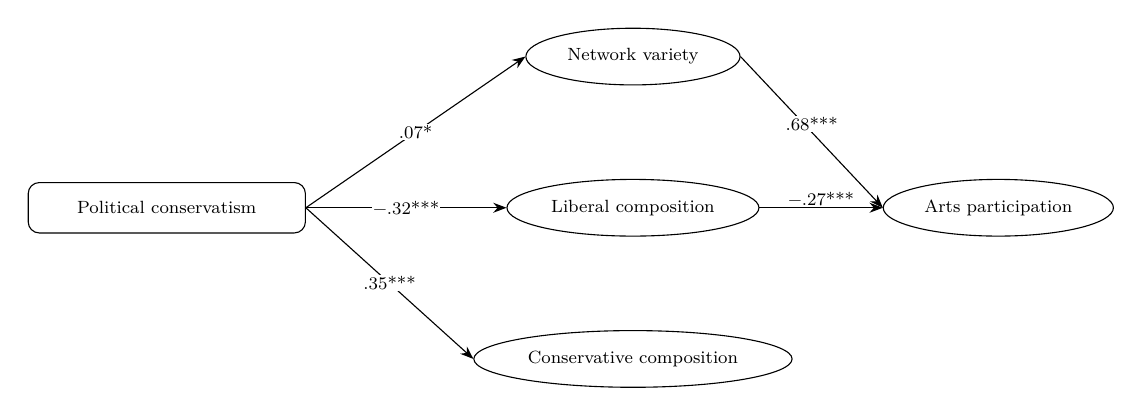
\begin{tikzpicture}[>=Stealth, font=\footnotesize, scale=0.8, transform shape,
  box/.style={draw, rounded corners, align=center, minimum width=4.4cm, minimum height=0.8cm},
  lat/.style={draw, ellipse, align=center, minimum width=3.4cm, minimum height=0.9cm},
  lab/.style={fill=white, inner sep=0.5pt, font=\footnotesize}]
\node[box] (x) at (0,0) {Political conservatism};
\node[lat] (wv) at (7.4,2.4) {Network variety};
\node[lat] (wl) at (7.4,0) {Liberal composition};
\node[lat] (wc) at (7.4,-2.4) {Conservative composition};
\node[lat] (act) at (13.2,0) {Arts participation};

\draw[->] (x.east) -- node[lab, pos=0.5] {.07*} (wv.west);
\draw[->] (x.east) -- node[lab, pos=0.5] {$-$.32***} (wl.west);
\draw[->] (x.east) -- node[lab, pos=0.5] {.35***} (wc.west);
\draw[->] (wv.east) -- node[lab, pos=0.5, above] {.68***} (act.west);
\draw[->] (wl.east) -- node[lab, pos=0.5, above] {$-$.27***} (act.west);
\end{tikzpicture}
\end{center}

Note. Standardized coefficients from the strong-tie structural model (N = 1,227). Solid arrows are paths through the network factors, dashed arrows are direct paths, and only paths significant at p < .05 are drawn. Asterisks follow Table 6.

Table 11. Direct, Network-Mediated, and Total Standardized Effects of Education, Childhood Arts Exposure, and Political Ideology on the Activity Factors, Weak Ties

\begin{tabular*}{\textwidth}{@{\extracolsep{\fill}}>{\raggedright\arraybackslash}p{0.40\textwidth} >{\raggedleft\arraybackslash}p{0.16\textwidth} >{\raggedleft\arraybackslash}p{0.16\textwidth} >{\raggedleft\arraybackslash}p{0.16\textwidth}@{}}
\toprule
Effect & Arts & Solitary leisure & Residual \\
\midrule
\textit{Education (ordinal)} & & & \\
\quad Direct & \hphantom{$-$}0.20***\hphantom{} & \hphantom{$-$}0.32***\hphantom{} & \hphantom{$-$}0.06\hphantom{***} \\
\quad Network-mediated & \hphantom{$-$}0.18***\hphantom{} & \hphantom{$-$}0.04\hphantom{***} & \hphantom{$-$}0.20***\hphantom{} \\
\quad Total & \hphantom{$-$}0.38***\hphantom{} & \hphantom{$-$}0.37***\hphantom{} & \hphantom{$-$}0.26***\hphantom{} \\
\textit{Childhood arts exposure} & & & \\
\quad Direct & \hphantom{$-$}0.16***\hphantom{} & \hphantom{$-$}0.16***\hphantom{} & \hphantom{$-$}0.07\hphantom{***} \\
\quad Network-mediated & \hphantom{$-$}0.13***\hphantom{} & \hphantom{$-$}0.06**\hphantom{*} & \hphantom{$-$}0.12***\hphantom{} \\
\quad Total & \hphantom{$-$}0.29***\hphantom{} & \hphantom{$-$}0.22***\hphantom{} & \hphantom{$-$}0.19***\hphantom{} \\
\textit{Political ideology} & & & \\
\quad Direct & $-$0.12*\hphantom{**} & $-$0.01\hphantom{***} & $-$0.27**\hphantom{*} \\
\quad Network-mediated & \hphantom{$-$}0.20***\hphantom{} & $-$0.09\hphantom{***} & \hphantom{$-$}0.39***\hphantom{} \\
\quad Total & \hphantom{$-$}0.09***\hphantom{} & $-$0.10*\hphantom{**} & \hphantom{$-$}0.12***\hphantom{} \\
\bottomrule
\end{tabular*}

Note. Standardized effects from the weak-tie structural model (N = 1,227). Network-mediated effects sum the products of the demographic-to-network and network-to-activity paths across the three weak-tie network factors, and total effects equal direct plus indirect. * p < .05, ** p < .01, *** p < .001, using delta-method standard errors.


Table 12. Direct, Network-Mediated, and Total Standardized Effects of Education, Childhood Arts Exposure, and Political Ideology on the Activity Factors, Strong Ties

\begin{tabular*}{\textwidth}{@{\extracolsep{\fill}}>{\raggedright\arraybackslash}p{0.40\textwidth} >{\raggedleft\arraybackslash}p{0.16\textwidth} >{\raggedleft\arraybackslash}p{0.16\textwidth} >{\raggedleft\arraybackslash}p{0.16\textwidth}@{}}
\toprule
Effect & Arts & Solitary leisure & Residual \\
\midrule
\textit{Education (ordinal)} & & & \\
\quad Direct & \hphantom{$-$}0.25***\hphantom{} & \hphantom{$-$}0.32***\hphantom{} & \hphantom{$-$}0.16***\hphantom{} \\
\quad Network-mediated & \hphantom{$-$}0.13***\hphantom{} & \hphantom{$-$}0.05**\hphantom{*} & \hphantom{$-$}0.11***\hphantom{} \\
\quad Total & \hphantom{$-$}0.38***\hphantom{} & \hphantom{$-$}0.37***\hphantom{} & \hphantom{$-$}0.27***\hphantom{} \\
\textit{Childhood arts exposure} & & & \\
\quad Direct & \hphantom{$-$}0.16***\hphantom{} & \hphantom{$-$}0.16***\hphantom{} & \hphantom{$-$}0.10*\hphantom{**} \\
\quad Network-mediated & \hphantom{$-$}0.13***\hphantom{} & \hphantom{$-$}0.06**\hphantom{*} & \hphantom{$-$}0.09***\hphantom{} \\
\quad Total & \hphantom{$-$}0.29***\hphantom{} & \hphantom{$-$}0.22***\hphantom{} & \hphantom{$-$}0.19***\hphantom{} \\
\textit{Political ideology} & & & \\
\quad Direct & $-$0.04\hphantom{***} & $-$0.01\hphantom{***} & $-$0.10\hphantom{***} \\
\quad Network-mediated & \hphantom{$-$}0.13***\hphantom{} & $-$0.08\hphantom{***} & \hphantom{$-$}0.22***\hphantom{} \\
\quad Total & \hphantom{$-$}0.09***\hphantom{} & $-$0.09*\hphantom{**} & \hphantom{$-$}0.12***\hphantom{} \\
\bottomrule
\end{tabular*}

Note. Standardized effects from the strong-tie structural model (N = 1,227). Network-mediated effects sum the products of the demographic-to-network and network-to-activity paths across the three strong-tie network factors, and total effects equal direct plus indirect. * p < .05, ** p < .01, *** p < .001, using delta-method standard errors.



\subsection*{Appendix: Confirmatory Measurement Models}

Table A1. Standardized Loadings and Antonym Residual Covariances from the Separate Weak-Tie and Strong-Tie Confirmatory Models

\begin{tabular*}{\textwidth}{@{\extracolsep{\fill}}>{\raggedright\arraybackslash}p{0.36\textwidth} l >{\raggedleft\arraybackslash}p{0.12\textwidth} l >{\raggedleft\arraybackslash}p{0.12\textwidth}@{}}
\toprule
Item & Weak factor & Loading & Strong factor & Loading \\
\midrule
Asian people & Variety & 0.83 & Variety & 0.77 \\
Second home & Variety & 0.68 & Variety & 0.71 \\
Born elsewhere & Variety & 0.78 & Variety & 0.78 \\
Middle Eastern or North African people & Variety & 0.84 & Variety & 0.86 \\
Native Hawaiian or Pacific Islander people & Variety & 0.82 & Variety & 0.83 \\
American Indian people & Variety & 0.74 & Variety & 0.81 \\
LGBTQ people & Liberal & 0.69 & Liberal & 0.71 \\
Little church & Liberal & 0.67 & Liberal & 0.67 \\
Very liberal & Liberal & 0.71 & Liberal & 0.73 \\
Hispanic or Latine people & Liberal & 0.77 & Variety & 0.73 \\
Black people & Liberal & 0.76 & Variety & 0.76 \\
City people & Liberal & 0.70 & Liberal & 0.77 \\
Lots of church & Conservative & 0.83 & Conservative & 0.83 \\
Very conservative & Conservative & 0.73 & Conservative & 0.73 \\
White people & Conservative & 0.84 & Conservative & 0.78 \\
Rural people & Conservative & 0.60 & Conservative & 0.62 \\
\midrule
Very liberal with very conservative & Residual & $-0.32$ & Residual & $-0.55$ \\
Little church with lots of church & Residual & 0.10 & Residual & $-0.05$ \\
City people with rural people & Residual & $-0.40$ & Residual & $-0.44$ \\
\bottomrule
\end{tabular*}

Note. Standardized loadings from separate three-factor WLSMV confirmatory models for weak ties and strong ties (N = 1,258 each), with the baseline models for the loadings. The residual rows come from the antonym-freed models, and each has a standard error of .02. Gender items are excluded. Item labels are abbreviated from the variable names and should be checked against the question wording.


\end{document}
